% !TeX root = ./paper.tex
\documentclass[modern]{aastex62}

% Load the corTeX style definitions
% !TeX root = ./ms.tex
% All the packages
\usepackage{url}
\usepackage{amsmath}
\usepackage{mathtools}
\usepackage{amssymb}
\usepackage{natbib}
\usepackage{graphicx}
\usepackage{calc}
\usepackage{etoolbox}
\usepackage{xspace}
\usepackage[T1]{fontenc} % https://tex.stackexchange.com/a/166791
\usepackage{textcomp}
\usepackage{ifxetex}
\ifxetex
\usepackage{fontspec}
\defaultfontfeatures{Extension = .otf}
\fi
\usepackage{fontawesome}
\usepackage{listings}
\usepackage{nicefrac}
\usepackage[bb=boondox]{mathalfa}
\usepackage{booktabs}
\usepackage{longtable}

% Shorthand for this paper
\newcommand{\starry}{\textsf{starry}\xspace}
\newcommand{\Python}{\textsf{Python}\xspace}
\newcommand{\cpp}{\textsf{C}++\xspace}
\newcommand{\bvec}[1]{{\ensuremath{\mathbf{#1}}}}
\newcommand{\xxx}[1]{{\color{red}#1}}
\DeclarePairedDelimiter\floor{\lfloor}{\rfloor}
\DeclarePairedDelimiter\ceil{\lceil}{\rceil}
\newcommand{\imag}{{\ensuremath{\mathbb{i}}}}
\newcommand{\quadquad}{\quad\quad\quad\quad}

\newcommand{\R}{\bvec{R}}
\newcommand{\AOne}{\bvec{A_1}}
\newcommand{\alm}{\bvec{a}}
\newcommand{\x}{\bvec{x}}
\newcommand{\D}{D}
\newcommand{\Doppler}{\bvec{D}}
\newcommand{\Surf}{\mathcal{S}}
\newcommand{\Curve}{\mathcal{C}}
\newcommand{\Dargs}{\bvec{d}}
\newcommand{\lmax}{\ensuremath{l_\mathrm{max}}}
\newcommand{\spot}{\texttt{SPOT}\xspace}
\newcommand{\vogtstar}{\texttt{VOGTSTAR}\xspace}
\newcommand{\kT}{\boldsymbol{\kappa}^\top}
\newcommand{\rhoT}{\boldsymbol{\rho}^\top}
\newcommand{\ylmbasis}{\boldsymbol{\psi}^\top}
\newcommand{\pbasis}{\boldsymbol{\phi}^\top}
\newcommand{\pbasisn}{\ensuremath{\phi_n}}
\newcommand{\azero}{\ensuremath{\bvec{a_0}}}

% References to text content
\newcommand{\documentname}{\textsl{article}}
\newcommand{\figureref}[1]{\ref{fig:#1}}
\newcommand{\Figure}[1]{Figure~\figureref{#1}}
\newcommand{\figurelabel}[1]{\label{fig:#1}}
\renewcommand{\eqref}[1]{\ref{eq:#1}}
\newcommand{\Eq}[1]{Equation~(\eqref{#1})}
\newcommand{\eq}[1]{\Eq{#1}}
\newcommand{\eqalt}[1]{Equation~\eqref{#1}}

% Add code, proof, and animation hyperlinks
\definecolor{linkcolor}{rgb}{0.1216,0.4667,0.7059}
\newcommand{\codeicon}{{\color{linkcolor}\faFileCodeO}}
\newcommand{\prooficon}{{\color{linkcolor}\faPencilSquareO}}
\newcommand{\codelink}[1]{\href{https://github.com/user/repo/blob/cfda45841cf4235e82cf705ab27251bd783bdf8c/tex/figures/#1.py}{\codeicon}\,\,}
\newcommand{\animlink}[1]{\href{https://github.com/user/repo/blob/cfda45841cf4235e82cf705ab27251bd783bdf8c/tex/figures/#1.gif}{\animicon}\,\,}
\newcommand{\prooflink}[1]{\href{https://github.com/user/repo/blob/cfda45841cf4235e82cf705ab27251bd783bdf8c/tex/proofs/#1.ipynb}{\raisebox{-0.1em}{\prooficon}}}
\newcommand{\cilink}[1]{\href{https://dev.azure.com/user/repo/_build}{#1}}


% Define a proof environment for open source equation proofs
\newtagform{eqtag}[]{(}{)}
\newcommand{\currentlabel}{None}
\newenvironment{proof}[1]{%
\ifstrempty{#1}{%
\renewtagform{eqtag}[]{\raisebox{-0.1em}{{\color{red}\faPencilSquareO}}\,(}{)}%
}{%
\renewtagform{eqtag}[]{\prooflink{#1}\,(}{)}%
}%
\usetagform{eqtag}%
\renewcommand{\currentlabel}{#1}
\align%
}{%
\endalign%
\renewtagform{eqtag}[]{(}{)}%
\usetagform{eqtag}%
\message{<<<\currentlabel: \theequation>>>}%
}

% Display the runtime on Azure
\usepackage[skins]{tcolorbox}
\newtcbox{\figtimebox}{enhanced,nobeforeafter,tcbox raise=-0.8mm,boxrule=0.6pt,
  top=0.5mm,bottom=0mm,right=0mm,left=6mm,arc=1pt,boxsep=2pt,
  before upper={\vphantom{dlg}},colframe=linkcolor,coltext=linkcolor,
  fontupper=\sffamily\bfseries\tiny,colback=white,overlay={\begin{tcbclipinterior}
  \fill[linkcolor] (frame.south west)
  rectangle node[text=white,font=\sffamily\bfseries\tiny,rotate=0]{CPU} 
  ([xshift=6mm]frame.north west);\end{tcbclipinterior}}}
\robustify{\figtimebox}
\pdfstringdefDisableCommands{%
  \def\figtimebox#1{'#1'}%
}
\newcommand{\figtime}[1]{\IfFileExists{figures/#1.py.time}%
{%
\cilink{\figtimebox{\input{figures/#1.py.time}\unskip s}}
}{}}

% Define the `oscaption` command for open source figure captions
\newcommand{\oscaption}[2]{\caption{#2 \codelink{#1} \figtime{#1}}}

% Code examples
\definecolor{codegreen}{rgb}{0,0.6,0}
\definecolor{codegray}{rgb}{0.5,0.5,0.5}
\definecolor{codepurple}{rgb}{0.58,0,0.82}
\definecolor{backcolour}{rgb}{0.95,0.95,0.95}
\lstdefinestyle{mystyle}{
    backgroundcolor=\color{backcolour},
    commentstyle=\color{codegreen},
    keywordstyle=\color{magenta},
    numberstyle=\tiny\color{codegray},
    stringstyle=\color{codepurple},
    basicstyle=\small\ttfamily,
    breakatwhitespace=false,
    breaklines=true,
    captionpos=b,
    keepspaces=true,
    numbers=left,
    numbersep=5pt,
    showspaces=false,
    showstringspaces=false,
    showtabs=false,
    tabsize=2,
    aboveskip=1em,
    belowskip=1em,
    keywords=[2]{map},
    keywordstyle=[2]{\color{black!80!black}},
    upquote=true
}
\lstset{style=mystyle}

% Typography obsessions
\setlength{\parindent}{3.0ex}
\renewcommand\quad{\hskip\fontdimen3\font}

% https://tex.stackexchange.com/a/184474
\usepackage{stackengine,scalerel}
\def\lnlam{\ThisStyle{\ensurestackMath{\stackon[-2.4\LMpt]{%
  \SavedStyle\lambda}{\kern-.5pt\kern\LMpt\rule{1\LMex}{.25pt+.15\LMpt}}}}}

% Bibliography stuff
\bibliographystyle{aasjournal}

% Begin!
\begin{document}

% Title
%\title{Inferring a time dependent map of Io's surface from occultations and phase curves.}
\title{Time-variable surface mapping of exoplanets: an application to Io}

% Author list
\author{Fran Bartoli\'c}
\email{fbartolic@flatironinstitute.org}
\affil{Center~for~Computational~Astrophysics, Flatiron~Institute, New~York, NY}
\affil{Centre for Exoplanet Science, SUPA, School of Physics and Astronomy, University of St. Andrews, St. Andrews, UK}
\author{Rodrigo Luger}
\author{Daniel Foreman-Mackey}
\affil{Center~for~Computational~Astrophysics, Flatiron~Institute, New~York, NY}
%

\begin{abstract}
Jupiter's moon Io is the most volcanically active body in the Solar System with hundreds of active volcanoes varying in intensity on different timescales.
Existing photometric observations in the near infrared taken during occultations by Jupiter and Galilean moons encode a wealth of information about its surface.
As such, Io is an ideal testbed for models of time-variable exoplanet surfaces.
We build a single probabilistic model of Io's surface using Nonnegative Matrix Factorization to infer one map per light curve.
The model is built on top of the code starry \href{https://rodluger.github.io/starry/}{\color{linkcolor}\faGithub} which can compute occultation light curves and phase curves in both emitted and reflected light. It also enables efficient inference with gradient based samplers.
We use the inferred map to study the time variability of prominent volcanoes over a timescale of decades.
While we mostly focus on Io, the lessons we learn are directly applicable to mapping exoplanets.
We discuss this application towards the end of the paper.\href{https://github.com/fbartolic/volcano}{\color{linkcolor}\faGithub}

\end{abstract}

%
\section{Introduction}
%% ADD PARAGRAPH REVIEWING PREVIOUS LITERATURE ON MAPPING EXOPLANETS, MENTION JWST AND LUVOIR
%% MAYBE EVEN IN THE ABSTRACT
The surface of Jupiter's moon Io is littered with hundreds of volcanoes appearing as bright spots in the near infrared and varying in intensity on timescales of days to decades.
The volcanic activity is driven by tidal interactions with Jupiter and sustained by the Laplace resonance with Europa and Ganymede \citep{peale_melting_1979}.
Io is a perfect analogue of an extremely volcanically active exoplanet.
Such rocky exoplanets, often dubbed \emph{super-Ios} or \emph{lava worlds}, have gathered a lot of interest in recent years because the photometric and spectral signatures of volcanic activity on such worlds will likely be detectable in the near future \citep{kaltenegger_detecting_2010,henning_highly_2018,oza_sodium_2019}.
Studying volcanism on both Io and exoplanets is scientifically valuable because it provides a window into the properties of early Earth and it informs theories of planet formation.

Existing exoplanet detections with potential volcanism include CoRoT-7b \citep{barnes_corot-7b_2010}, the first discovered rocky exoplanet with likely significant tidal heating; 55 Cancri e, whose longitudinal offset in peak surface emission has been attributed to, among other things, lava flows on the surface \citep{demory_variability_2016,demory_map_2016,hammond_linking_2017}; several planets in the TRAPPIST-1 system in a Laplace-like resonance with likely volcanic activity \citep{kislyakova_magma_2017,dobos_tidal_2019}; and many others.
Not all exoplanets will have Io-like volcanism, some will have magma oceans due to their proximity to the star or volcanism caused by nuclear decay similar to early Earth volcanism.

Io has been observed extensively using both space and ground observatories.
High resolution images of Io's surface were taken by space missions such as Voyager \citep{smith_jupiter_1979}, Galileo \citep{belton_galileos_1996} and Juno \citep{mura_infrared_2020}.
It has also been resolved from the ground in the near infrared using disk resolved imaging
\citep{howell_infrared_1985,simonelli_disk-resolved_1986,spencer_discovery_1990} and adaptive optics observations \citep{marchis_adaptive_2000,marchis_keck_2005,de_kleer_spatial_2016}.
Most importantly for this work, Io has been sporadically observed for decades using high cadence near infrared photometry taken during occultations by Jupiter starting with \cite{spencer_discovery_1990}.
Occultations by Jupiter occur twice every orbit lasting ~1.7 days and mutual occultations with Europa, Ganymede or Callisto happen every ~6 years when Earth pasess through the orbital plane of Galilean satellites.
The majority of occultations by Jupiter are observed when Io is in Jupiter's shadow ("in eclipse") while mutual occultations are almost always observed in sunlight because mutual occultations while Io is in eclipse are extraordinarily rare.
Only the brightest volcanoes are visible over the reflected light background when Io is illuminated by the Sun\citep{veeder_ios_1994,de_kleer_spatial_2016}.

Both kinds of occultations have been used to study volcanic activity on the surface.
\cite{spencer_io_1994} observed several occultations of Io by Europa and detected a major brightening of the most powerful of Io's volcanoes, Loki, relative to previous Voyager observations.
\cite{rathbun_loki_2002, rathbun_loki_2006,rathbun_ground-based_2010} used observations from NASA's IRTF telescope to study the long term variability of different volcanic spots finding evidence of periodicity in Loki's eruptions and established the transient nature of the volcanoes (only Loki is persistently active).
By studying an occultation of Io by Europa, \cite{de_kleer_multi-phase_2017} mapped the Loki region to a precision of about 2 kilometers.
In addition to observations of occultations in near infrared, several groups have been observing mutual occultations in the optical \citep[][and references therein]{arlot_mutual_1974,saquet_phemu15_2018,morgado_astrometry_2016} with the purpose of inferring the optical albedo of Io and improving ephemeris precision for Galilean satellites.

None of the studies of occultations in the infrared attempted to infer a two-dimensional map of Io's surface.
The light curves are usually fit independently with the goal of inferring one-dimensional longitudinal variations in brightness on its surface.
Strong priors on the locations of individual volcanoes are assumed based on maps from space mission observations.
In this work, we build a fully probabilistic model in order to infer a time-dependent two-dimensional \emph{map} of Io's volcanic surface from archival IRTF observations in the near infra red.
The model is built on top of the recently developed code starry \citep[][Luger et al. 2020 in prep]{luger_starry_2019} which
enables fast analytic computation of occultation light curves and phase curves for objects whose surface features are represented in terms of spherical harmonics.
starry can compute phase curves and occultations in both emitted light (for modeling the isotropic volcanic emission from Io's surface) and reflected light (for mapping albedo variations).
Instead of fitting one map per occultation light curve, we reduce the dimensionality of the problem using matrix factorization, assuming a fixed map for a given light curve which is a linear combination of $K$ basis maps.
We use priors on the map features which ensure the maps are physical and prevent overfitting of the data.
The model is interpretable, each of the basis maps roughly corresponds to a single spot on the surface, and the coefficients multiplying the basis maps encode information on the time variability.

Our goals for this paper are to both improve on past studies of Io using occultation light curves and to construct a flexible model directly applicable to future efforts on inferring time-dependent maps of variable features on exoplanet surfaces such as volcanoes, magma oceans or clouds.
The fact that we have lots of prior information on what the surface of Io should look like enables us to test our model in a realistic setting, testing sensitivity to chosen priors, data quality, the orbital parameters and different kinds of surface features.

The paper is organized as follows.
In \S\ref{sec:data} we describe the IRTF light curves of occultations by Jupiter which we use to infer maps.
In \S\ref{sec:model} we discuss the generative model for the data for the case of a static map, and a dynamic map modeled using a matrix factorization approach and we write down the relevant likelihood functions.
In \S\ref{sec:inverse_problem} we focus on the question of how to do Bayesian inference given the forward model specifications defined in \S\ref{sec:model}.
We discuss and test different priors on map features, the information content of light curves and fitting the models using variational inference (VI) methods and Hamiltonian Monte Carlo (HMC).
We present results on simulated data.
\S\ref{sec:results} shows the results on real data.
In particular, the inferred dynamic map, the  different component maps and accompanying coefficients, the uncertainties of the maps, sensitivity to different choices of priors, comparison of inferred locations and intensities of spots to known values from the literature.
Finally, in \S\ref{sec:exoplanets} we discuss applications of the model to future exoplanet obervations and test the model predictions on simulated JWST observations of a volcanic Super-Earth.

\section{Data}
\label{sec:data}

\begin{figure}[h!]
    \begin{centering}
    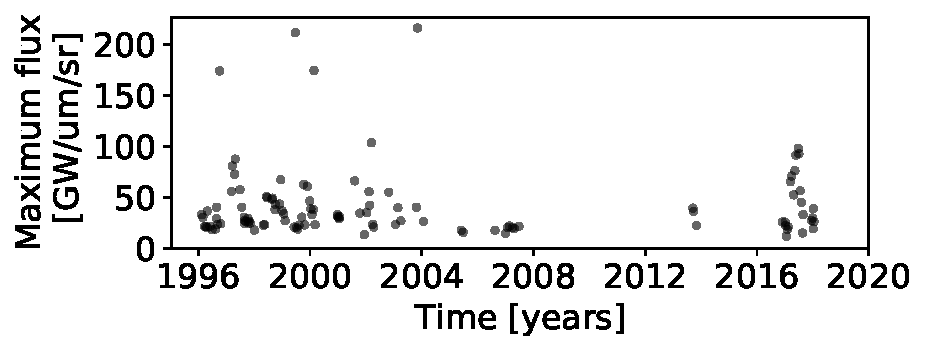
\includegraphics[width=0.5\linewidth]{figures/irtf_max_flux.pdf}
    \oscaption{irtf_dataset}{%
        Maximum flux for each curve taken using NASA's IRTF telescope during an
        occultation of Io by Jupiter.
       \label{fig:irtf_max_flux}
    }
    \end{centering}
\end{figure}

The dataset we use to infer maps of Io's surface consists of 112 observations of Io in the near infrared taken from 1996 until 2018 using various instruments at NASA's IRTF observatory.
Figure~\ref{fig:irtf_max_flux} shows the maximum flux in $\mathrm{GW}/\mu \mathrm{m}/\mathrm{sr}$ for each light curve plotted as a function of time which approximately corresponds to the disc integrated flux of Io at the beginning of ingress or the end of egress prior to it being occulted by Jupiter.
Two features of this plot are apparent.
First although the observations span decades the cadence is non-uniform with only a few observations taken between 2008 and 2016.
Second, the baseline brightness is varying stochastically by a large amount and there are several notable events of increased volcanic activity.
All of the observations were taken while Io was \emph{in eclipse}, meaning that it was in Jupiter's shadow and all of the observed emission from the surface is due to thermal radiation.
Observations of Io \emph{in sunlight} on the other hand probe both the thermal (volcanic) emission and the surface albedo variations in the near infrared.


\begin{figure}[h!]
    \begin{centering}
    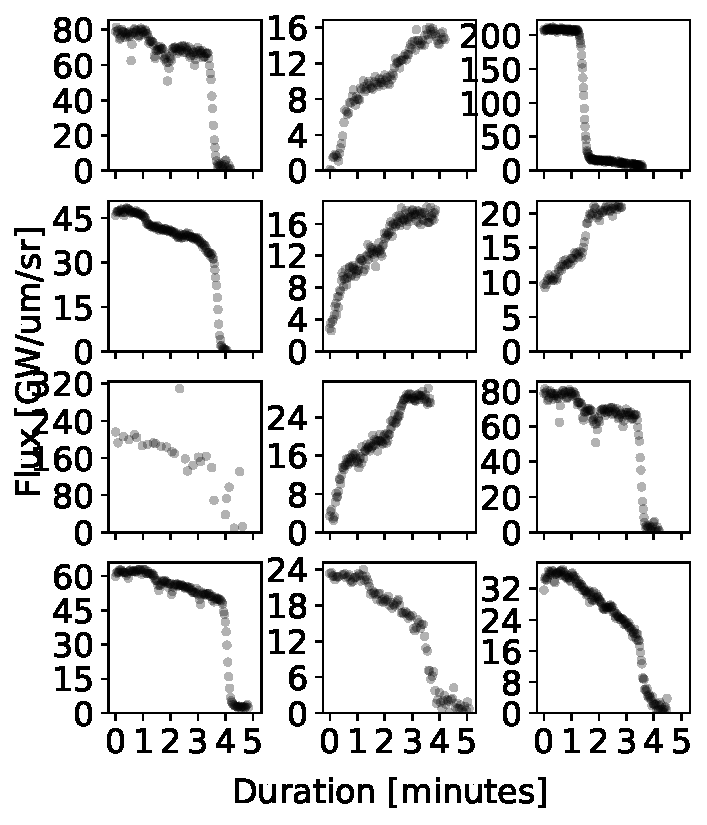
\includegraphics[width=0.5\linewidth]{figures/irtf_sample_lightcurves.pdf}
    \oscaption{irtf_dataset}{%
        A selection of sample light curves taken during occultations of Io by Jupiter in our dataset.
        The step-like morphology of the light curves is due to bright volcanoes on Io's surface coming in or out of view during an occultation.
        These light curves thus visibly encode information about the features on the surface.
        \label{fig:irtf_sample_lightcurves}
    }
    \end{centering}
\end{figure}

In Figure~\ref{fig:irtf_sample_lightcurves} we display a random subset of all the light curves
in the dataset.
All occultations last for $\sim4$ min and the cadence for each light varies but it on the order of a second.
It follows that over the course of a single exposure Jupiter's limb move by about 15km which provides a lower bound for the size of the features on the surface that we can reliably estimate.
The shapes of light curves strongly deviate from the smooth variability one would expect assuming a homogeneous distribution of thermal emission on the surface.
Especially prominent are light curves with clear step-like features which are present when bright spots come in or out of view during the course of an occultation.
The fact that these features are so clearly visible means that even individual light curves encode a wealth of information about the surface.

The photometric quality varies from year to year because multiple instruments were used over the years.
An additional issue is that estimated errorbars aren't provided.
As with all ground based photometry, the observations are influenced by atmospheric variability which induces correlated noise in the light curves.
Because of this the flux isn't always monotonically increasing or decreasing as one would expect.
All of these issues need to be accounted for in the final model.

\section{Model}
\label{sec:model}
% Discuss starry, pixels vs. schmixels vs. harmonics, forward model for static map, NMF model for dynamic map
\subsection{Orbital parameters}
\label{ssec:orbital_parameters}
To model the occultations we need to know the projected separation between Jupiter and Io and the orientation of Io at any given time.
We use the \href{https://ssd.jpl.nasa.gov/horizons.cgi}{JPL Horizons database} and the latest planetary ephemeris DE430 \citep{folkner_planetary_2014} for this purpose.
Specifically, we use the Right Ascension and Declination, the angular (equatorial) diameter (\textsf{Ang-diam}), the visibility flag indicating whether Io is occulted or not and whether it is in partial or total eclipse (\textsf{Ang-sep/v}), the longitude and latitude at the center of Io's disc as seen from Earth (\textsf{Ob-lon}, \textsf{Ob-lat}), the sub-solar point longitude and latitude which specify the direction pointing towards the Sun on Io's surface (\textsf{Sl-lon}, \textsf{Sl-lat}), the distance from Io to the Sun (\textsf{r}) and
the counterclockwise angle between the Celestial North Pole unit vector projected onto the plane of the sky and the Io's north pole (\textsf{NP.ang}).
All longitudes are positive to the west.
\textsf{HORIZONS} provides all ephemeris with a minimum cadence of 1 second so we interpolate all values such that we can evaluate them for arbitrary times.

The coordinate system in \textsf{starry} is defined to be right handed such that the $\hat{z}$
axis points towards the observer and the $\hat{x}$ axis points to the right on the plane of the sky.
The radius of the occulted sphere is fixed to 1 and the orientation is specified by three angles,
the counterclockwise obliquity angle \textsf{obl} between the $\hat{y}$ axis and the North Pole of the sphere, the inclination angle \textsf{inc} which is set to $90^\circ$ if the North Pole is aligned with the $\hat{y}$ axis and the phase angle \textsf{theta} rotates the sphere around the $\hat{y}$ axis in the eastward direction.
We have $\mathrm{obl}=\textsf{NP.ang}$, $\mathrm{inc}=90^\circ-\textsf{Ob-lat}$ and
$\mathrm{theta}=\textsf{Ob-lon}$.
The occultor position relative to the occulted object is given by
\begin{align}
    \mathrm{xo}/\gamma&=-\Delta\alpha\,\cos\delta\\
    \mathrm{yo}/\gamma&=\Delta\delta\\
    \mathrm{zo}/\gamma&=1
\end{align}
where $\Delta\alpha$ are the $\Delta\delta$ differences in Right Ascension and Declination respectively relative to the occulted object and $\gamma$ is the angular radius of the occulted sphere.
If the occulted object is illuminated by the Sun then we also need to specify the coordinates of the light source which are given by
\begin{align}
    \mathrm{xs}&=r\cos\theta\sin\phi\\
    \mathrm{ys}&=r\sin\theta\\
    \mathrm{zs}&=r\cos\theta\cos\phi
\end{align}
where $\theta$ is obtained by subtracting \textsf{Ob-lat} from \textsf{Sl-lat} and similarly $\phi$ is obtained by subtracting \textsf{Ob-lon} from \textsf{Sl-lon}.
$r$ is equal to the heliocentric distance of the occulted object \textsf{r}.

\subsection{Static map model}
\label{ssec:static}
Given the geometry of on occultation event at an arbitrary time, computing the predicted flux with \textsf{starry} is straightforward.
\textsf{starry} computes the integrated flux of an unocculted or an occulted sphere analytically assuming that the surface map can be expanded in terms of spherical harmonics $Y_{lm}(\theta,\phi)$ up to a certain \emph{degree} $l$.
The map is thus defined by a vector of spherical harmonic coefficients $\mathbf{y}$ multiplying the spherical harmonic basis $\tilde{\mathbf{y}}(x, y)=\left(Y_{0,0} Y_{1,-1} Y_{1,0} Y_{1,1} Y_{2,-2} Y_{2,-1} Y_{2,0} Y_{2,1} Y_{2,2} \cdots\right)^{\top}$ and the total number of coefficients is $(l+1)^2$.
In addition to computing \emph{thermal} phase curves and occultation light curves, \textsf{starry} also solves the considerably more complex problem of computing reflected light phase curves and occultations when the sphere is illuminated by a distant light source \citep[Luger et al. 2020 in prep][]{} which is complicated by the presence of the terminator line.
In the case of a reflected light map, the coefficient vector $\mathbf{y}$ represents spherical albedo in a given wavelength range.
Most importantly, conditional on the parameters specifying the geometry of the occultations being fixed, the \textsf{starry} model is \emph{linear} for both emitted and reflected light maps.
This is achieved by representing all rotations, changes of basis and integrals with complicated boundaries needed to compute the flux as linear transformations.
Since a sequence of linear mappings is also linear, the predicted flux can be written as
\begin{equation}
    \mathbf{f}=\mathbf{A}\,\mathbf{y}
\end{equation}
where the column vector $\mathbf{f}$ of shape $(T, 1)$ is the predicted flux for different values of the occultor position and optionally the direction of the illumination source and $\mathbf{A}$ is the design
matrix of shape $(T, N)$ (with $N=(l+1)^2$) which encodes information all operations needed to compute the integrated flux.
If the geometry isn't known precisely then the matrix $\mathbf{A}$ is not fixed and the model is no longer linear.

The characteristic angular scale of features that can be represented with a given map is set by the degree of the map and it is approximately equal to $\frac{180^\circ}{l}$.
State of the art inferences involving phase curves and secondary eclipses of exoplanets are able to constrain features of order $l=1$ (inferring a bright spot on single hemisphere) but for Io we need to fit much higher order maps because the typical scale of volcanic spots is on the order of tens of kilometers (a few degrees).
\textsf{starry} can handle computations with maps up to $l\approx 20$ before numerical instabilities kick in (TODO: make this statement more precise).

Although \textsf{starry} is built around the idea of expending surface features in a spherical harmonic basis, this is not the ideal basis for doing inference because it makes it difficult to ensure positivity of the maps.
Ideally we would like to fit all models in the \emph{pixel basis} where ensuring positivity is trivial but still do all computations in the $Y_{lm}$ basis where everything is analytic and fast.
We obtain the pixels by constructing a discrete grid on the surface of the sphere using an equal area Molleweide projection.
To ensure that the intensity is positive everywhere on the surface we also need to have more pixels than spherical harmonics (by a factor of a few).
The mapping $\mathbf{P}$ from the spherical harmonic basis to the pixel basis is linear operator and it is straightforward to compute.
Unfortunately, because the number of pixels is greater than the number of $Y_{lm}$ coefficients, the matrix $\mathbf{P}$ is not square and is therefore not invertible.
We can still compute Moore-Penrose pseudoinverse $\mathbf{P}^\dagger$ which is obtained by solving the linear system $\mathbf{P}\,\mathbf{y}=\mathbf{p}$ where $\mathbf{p}$ is the vector of all pixels comprising a map.
The model is also linear in the pixels:
\begin{equation}
    \mathbf{f}=\mathbf{A}\,\mathbf{P}^\dagger\,\mathbf{p}
    \label{eq:linear_model_pix}
\end{equation}
In what follows, we will assume that we work in the pixel basis and compute all fluxes in the $Y_{lm}$ basis where the model is exact.
We will discuss the validity of this approach in detail in Section~\ref{sec:inverse_problem}.

\subsection{Nonnegative Matrix Factorization}
\label{ssec:nmf}
In the case when we cannot assume a static map, the situation is considerably more complicated.
In principle, the surface map is different for each \emph{data point}.
Of course, fitting one map per data point is intractable so we might instead fit a single map per light curve, generated by Eq.~\ref{eq:linear_model_pix}.
Even then, we would need to fit on the order of 1k parameters!
This is both becuse the number of spherical coefficients scales as $(l+1)^2$ and because when fitting in pixel space we need many more pixels than spherical harmonics to ensure positivity.
Although fitting a model of such high dimensionality for a single IRTF light curve of high signal to noise ratio is tractable thanks to exact gradients provided by autodifferentiation in \textsf{starry}, we don't want to do that for a hundred or so separate light curves.
Such a model would be very difficult to fit and it would require strong regularization between successive maps in time.
It also wouldn't directly provide much physical insight into the volcanic activity, we would have to conduct a separate analysis on the inferred maps to constrain the time variability of the volcanoes.
Instead, we need an approach which reduces the dimensionality of the problem.
One way of accomplishing that is to expand the spherical harmonic coefficients (or pixels) in a Taylor series in time about a certain point.
This is the approach \cite{luger_tess_2019} took to model a map of Earth's albedo in reflected light from stray Earthshine in the aperture of the TESS space telescope.
This issue with this approach and similar series expansions such as the Fourier series is that with the very long baseline of IRTF data and the observations being scattered throughout the years sporadically, it is unclear which point should be the origin of the expansion.
More importantly, there likely doesn't exist a well defined global time-averaged map of Io so requiring too much smoothness between successive maps wouldn't work.
Another way of reducing the dimensionality of the problem would be a parametric approach where where we place a few spots on the sphere and then fit only for the locations and intensities of each spot.
This is assuming that we know a priori that the surface features are spot like and roughly how many we should expect.
While such a strong assumption might work for studying individual spots in the context of Io, it certainly isn't justified for exoplanets.
In Section~\ref{sec:inverse_problem} we do assume stronger priors on the locations of and shapes of surface features to better constrain the variability of individual volcanoes, but we still fit for pixels, at least in principle allowing the data to override our assumptions.

The approach approach opted for is to treat the problem of inferring a single map per light curve as a probabilistic matrix factorization problem.
The idea is to assume that a map for any given light curve can be expressed as a linear combination of $K$ "basis maps".
Consider $L$ lightcurves, the model for the $l$-th light curve is
\begin{equation}
    \mathbf{f}_l=\mathbf{A}_l\,\mathbf{P}^\dagger\,\mathbf{p}_l
\end{equation}
We can stack the column vectors $\mathbf{p}_l$ into a matrix $\mathbf{Y}$ of shape $(N_p, L)$ where $N_p$ is the number of pixels for each light curve.
We then assume that the $\mathbf{Y}$ can be decomposed into a product of two matrices $\mathbf{B}$ and $\mathbf{Q}$ as
\begin{equation}
    \mathbb{Y}=\mathbf{B}\,\mathbf{Q}
    \label{eq:nmf}
\end{equation}
where $\mathbf{B}$ has shape $(N_p, K)$ and $\mathbf{Q}$ has shape $(K, L)$.
The model for all light curves can be written as
\begin{equation}
    \mathbb{f}=\mathbb{A}\,\mathrm{vec}(\mathbf{\mathbb{Y}})
    \label{eq:model_all_lcs}
\end{equation}
Where $\mathbf{f}$ is a tall column vector consisting of predictions for all light curves stacked together, $\mathbb{A}$ is a block diagonal matrix with matrices $\mathbf{A}_l\,\mathbf{P}^\dagger$ on the diagonal for $l=1\dots, L$ and the $\mathrm{vec}$ operator stacks the columns of $\mathbb{Y}$ into a tall vector.
The model is \emph{bilinear} which means that is linear in the matrices $\mathbb{B}$ and $\mathbf{Q}$ separately.
The interpretation of Equation~\ref{eq:nmf} is simple, each of the $K$ columns of $\mathbf{B}$ represents pixels of a basis map and the columns of $\mathbf{Q}$ determine how those maps add together to produce a final map for the $l$-th light curve.
Ideally, we want the basis maps to be physically meaningful and the coefficients encode the time variability.
A nice feature of this model is that there is no requirement that successive maps are smoothly varying between different light curves.

The matrix factorization problem as written in Equation~\ref{eq:nmf} is highly degenerate and practically intractable a probabilistic framework with a small dataset.
Since each of the columns of $\mathbf{B}$ are pixels representing emitted light or albedo, we can substantially reduce the ambiguity in the decomposition by requiring that both matrices are strictly positive.
This matrix factorization problem is known as \emph{Nonnegative Matrix Factorization} (NMF) \citep{paatero_positive_1994,lee_algorithms_2001} and it has a rich history across many different fields.
It is commonly used for decomposing physical signals in the spectral or the time domain.
Even though NMF is more tractable than unconstrained matrix factorization, it is still an NP hard problem \citep{vavasis_complexity_2009} and it requires additional constraints or priors to be tractable.
Simultaneously transforming $\mathbf{B}\leftarrow \mathbf{B}\,\mathbf{S}^{-1}$ and
$\mathbf{Q}\leftarrow \,\mathbf{S}\mathbf{Q}$ with a nonsingular matrix $\mathbf{S}$ doesn't change the value of the objective function.
The objective function is also invariant to a simultaneous permutation of the columns of $\mathbf{B}$ and rows of $\mathbf{Q}$ and rescaling either of the two matrices by a scalar.
Nevertheless, getting around these degeneracies in practice is possible, especially when we have a lot of prior knowledge on the problem.
For a recent review article with a detalied analysis of these degeneracies and common algorithms, see \cite{fu_nonnegative_2019}.


Broadly speaking, there are two approaches to fitting NMF models, the constrained optimization approach and the probabilistic approach.
In the optimization approach we optimize $\mathbb{Y}$ in a least-squares sense under a set of constraints on either one or both of the matrices \citep[see][for recent examples from the astronomical literature]{acosta-pulido_new_2017, melchior_scarlet_2018,ren_non-negative_2018,ren_using_2020}.
The probabilistic approach introduces priors and the inference is usually done with variational inference.
In this work we opt for the probabilistic approach because we care about the uncertanties on the map features a lot.

One difference between most applications of NMF in the literature and NMF within the context of infering surface maps from 1D light curves is that
in the majority of the work in the literature \citep[except][]{kawahara_global_2020} the matrix $\mathbb{Y}$ is assumed to be directly observed  up to a simple noise term.
In our case the problem is considerably more challenging because we observe the light curves
$\mathbb{A}\,\mathrm{vec}(\mathbf{\mathbb{Y}})$ instead of $\mathbb{Y}$ directly, a process in which some information is lost because, depending on the geometry of the occultations, certain combinations of spherical harmonic coefficients will be in the nullspace.
\cite{kawahara_global_2020} are using NMF to model phase variations in directly imaged exoplanets with the goal of simultaneously inferring a surface map and a spectral decomposition of the map into several components, a case in which the
matrix which is to be decomposed is also unobserved.
Although we don't attempt to solve the problem of spectrally decomposing the maps, our approach is directly applicable to that problem as well. (TODO: should I add more details here?)
One could also imagine inferring a multi spectral component and time dependent map by solving two NMF problems simultaneously.
We leave this application for future work.


\subsection{The likelihood}
\label{ssec:likelihood}
Given Eq.~\ref{eq:nmf} we can write down the likelihood for our data and in Section~\ref{sec:inverse_problem} we dicuss in detail the priors which make the problems of inferring static and dynamic maps tractable.
Assuming a Gaussian noise process for the data with a dense covariance matrix, the (log) likelihood is
\begin{equation}
    \ln\mathcal{L}=-\frac{1}{2}\left[\mathbb{f}_\mathrm{obs}-(\mathbb{f} + \mathbb{b})\right]^{\top} \boldsymbol{\Sigma}^{-1}\left[\mathbb{f}_\mathrm{obs}-(\mathbb{f} + \mathbb{b})\right]
\end{equation}
where $\mathbb{f}_\mathrm{obs}$ is the vector of stacked observed light curves, $\boldsymbol{\Sigma}$ is the data covariance matrix and $\mathbb{b}$ is a fixed flux offset per light curve accounting for stray flux not attributed to Io (mostly due to Jupiter).
We model the data covariance with a Gaussian Process using the fast Celerite method\citep{foreman-mackey_fast_2017} as implemented in the \textsf{exoplanet} package (TODO: cite) to capute correlations imposed by the seeing plus an additional white noise term which is different for each light curve.
The IRTF data isn't provided with any uncertainties so we estimate the uncertainties by filtering the data with the Savitzky Golay filter as implemented in \textsf{SciPy} (TODO: CITE) and estimating the variance of the residuals.
We assume identical errors for all data points in a given light curve but allow for a rescaling factor when fitting the model.
In the next section, we add priors to this likelihood and fit the model on simulated data using optimization and Variational Inference (VI).

%TODO: mention that A depends on the geometry and that we fit for some of those parameters.

\section{The inverse problem}
\label{sec:inverse_problem}
% bulk of the results in the paper
\subsection{The information content of a light curve}
\label{ssec:information_content}
% information in different kinds of occultations/phase curves, reflected light vs. emitted light, posterior shrinkage etc.

\begin{figure}[h!]
    \begin{centering}
    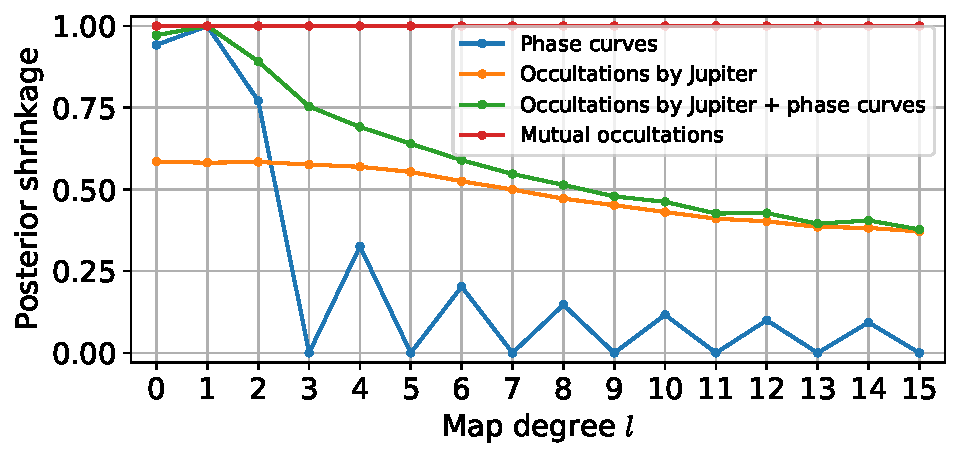
\includegraphics[width=0.5\linewidth]{figures/information_content.pdf}
    \oscaption{InformationContent}{%
        This is a plot of a pretty function. And at the end of this
        caption is a symbol with a link to the \emph{exact} script
        that generated it, hosted on \textsf{GitHub}.
        \label{fig:information_content}
    }
    \end{centering}
\end{figure}

\subsection{Fitting a static map}
\label{ssec:static_map}
% Priors for static maps, sparsity, positivity, plot of map inference with simulated data and different kinds of priors. Inference with MAP, VI, HMC.

\subsection{Fitting a dynamic map}
\label{ssec:dynamic_map}
% Priors for NMF. Optimization vs. bayesian approach to NMF. Results on simulated data. Comparison of results to matrix factorization without the positivity constraint and clever priors.

\section{Results}
\label{sec:results}

\subsection{Individual events}
\label{ssec:individual}
% Fits of individual events. In particular, those light curves that were analyzed in previous papers.

\begin{figure}[h!]
    \begin{centering}
    \includegraphics[width=1.\linewidth]{figures/single_event_fit.pdf}
    \oscaption{single_event_fit}{%
        This is a plot of a pretty function. And at the end of this
        caption is a symbol with a link to the \emph{exact} script
        that generated it, hosted on \textsf{GitHub}.
        \label{fig:single_event_fit}
    }
    \end{centering}
\end{figure}

\subsection{The time-variable map}
\label{ssec:time_variable_map}
%

\subsection{Variability of known hotspots}
\label{ssec:variability_hotspots}
% Plot inferred intensities of known hotspots as function of time, reference previous work.

\section{Mapping volcanic exoplanets}
\label{sec:exoplanets}
% Application to exoplanets. Fitting mock JWST observations.

\section{Conclusions}
\label{sec:conclusions}

% Bibliography
\bibliography{bib}
\end{document}
